\subsubsection{Critique sur le dimensionnement du filtre passe-haut}

Lors du dimensionnement du filtre passe-haut, nous n'avons pas pris en compte la résistance de polarisation de $2.2 \ k \Omega$ du microphone piézoélectrique, ni le filtre passe-bas de l'alimentation. Pour savoir si tout ceci modifie grandement les caractéristiques de notre filtre passe-haut, nous avons réalisé trois simulations sur LTspice. La première dont le schéma est visible sur la figure \ref{fig:ltspice_ideal}, simule un cas \textit{idéal}, sans prise en compte des filtres passe-bas et de la polarisation du microphone. La deuxième, sur la figure \ref{fig:ltspice_current}, simule le cas \textit{courant équivalent}, où les filtres passe-bas ne sont pas modélisés et le microphone et la polarisation sont remplacées par des source de courant\footnote{Les paramètres des sources ont été ajustés de façon à obtenir une réponse transitoire, voir Annexe \ref{LTspiceCurrentvsJFTTransient}, et une courbe de Bode satisfaisante}. La dernière simulation, \textit{équivalent transistor}, visible sur la figure \ref{fig:ltspice_transistor} propose un modèle plus proche de la réalité du microphone. Dans ce dernier cas, les filtres passe-bas sont simulés.

\begin{figure}[H]
    \centering
    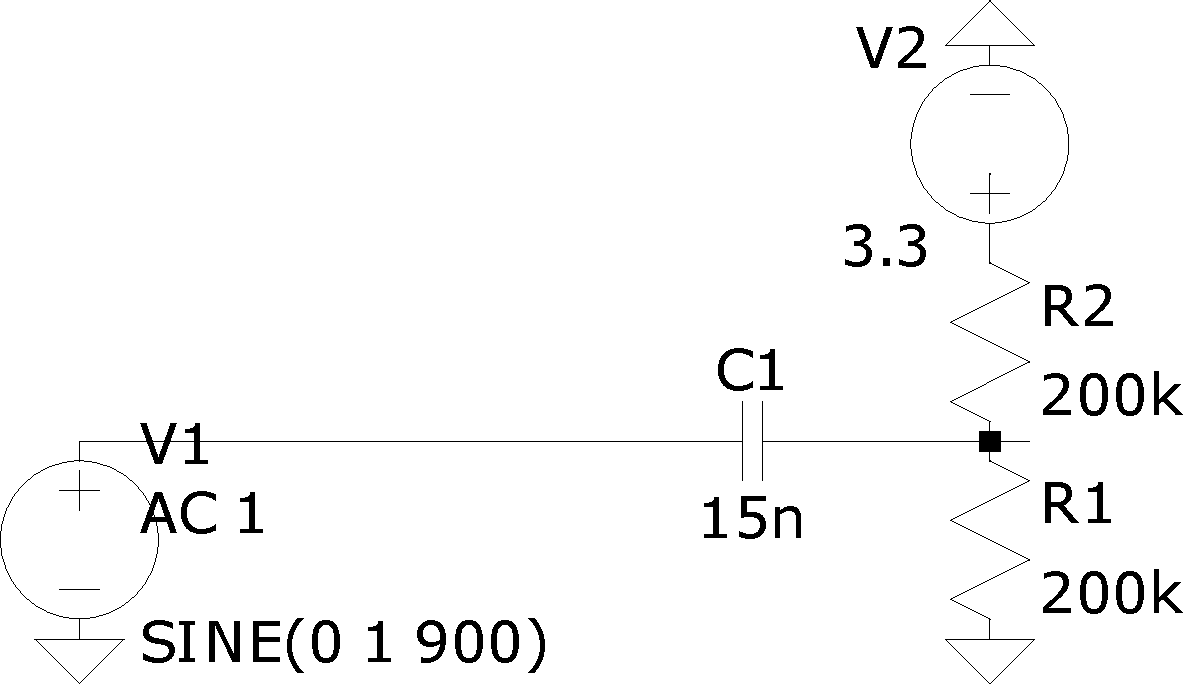
\includegraphics[width=0.3\textwidth]{pdffiles/HighPass/CircuitHighPassPolarization200k.pdf}
    \caption{Schéma de simulation sur LTspice du cas \textit{idéal}}
    \label{fig:ltspice_ideal}
\end{figure}
\begin{figure}[H]
    \centering
    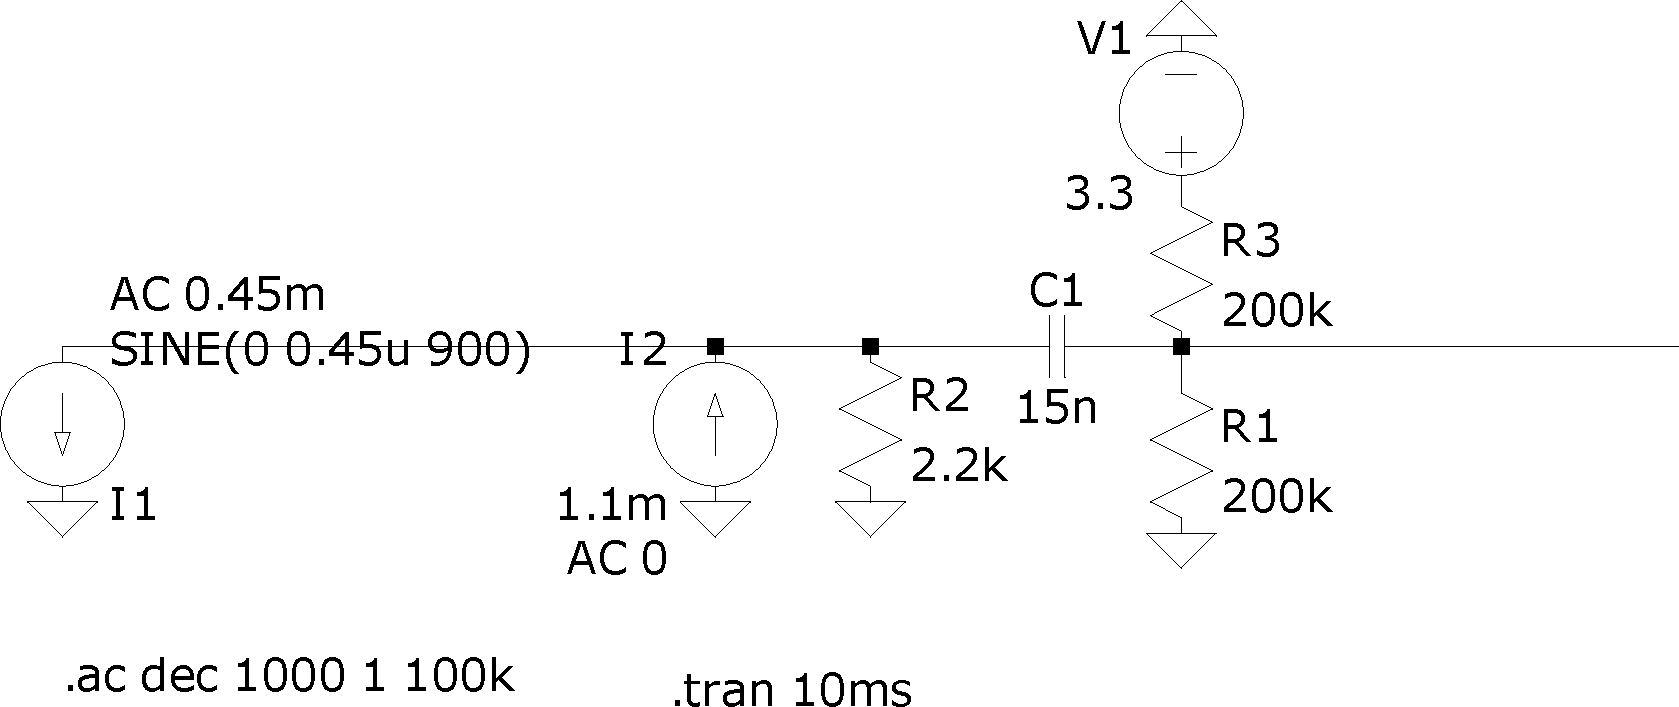
\includegraphics[width=0.4\textwidth]{pdffiles/HighPass/CircuitHighPassSimulationCurrent.pdf}
    \caption{Schéma de simulation sur LTspice du cas \textit{équivalent courant}}
    \label{fig:ltspice_current}
\end{figure}
\begin{figure}[H]
    \centering
    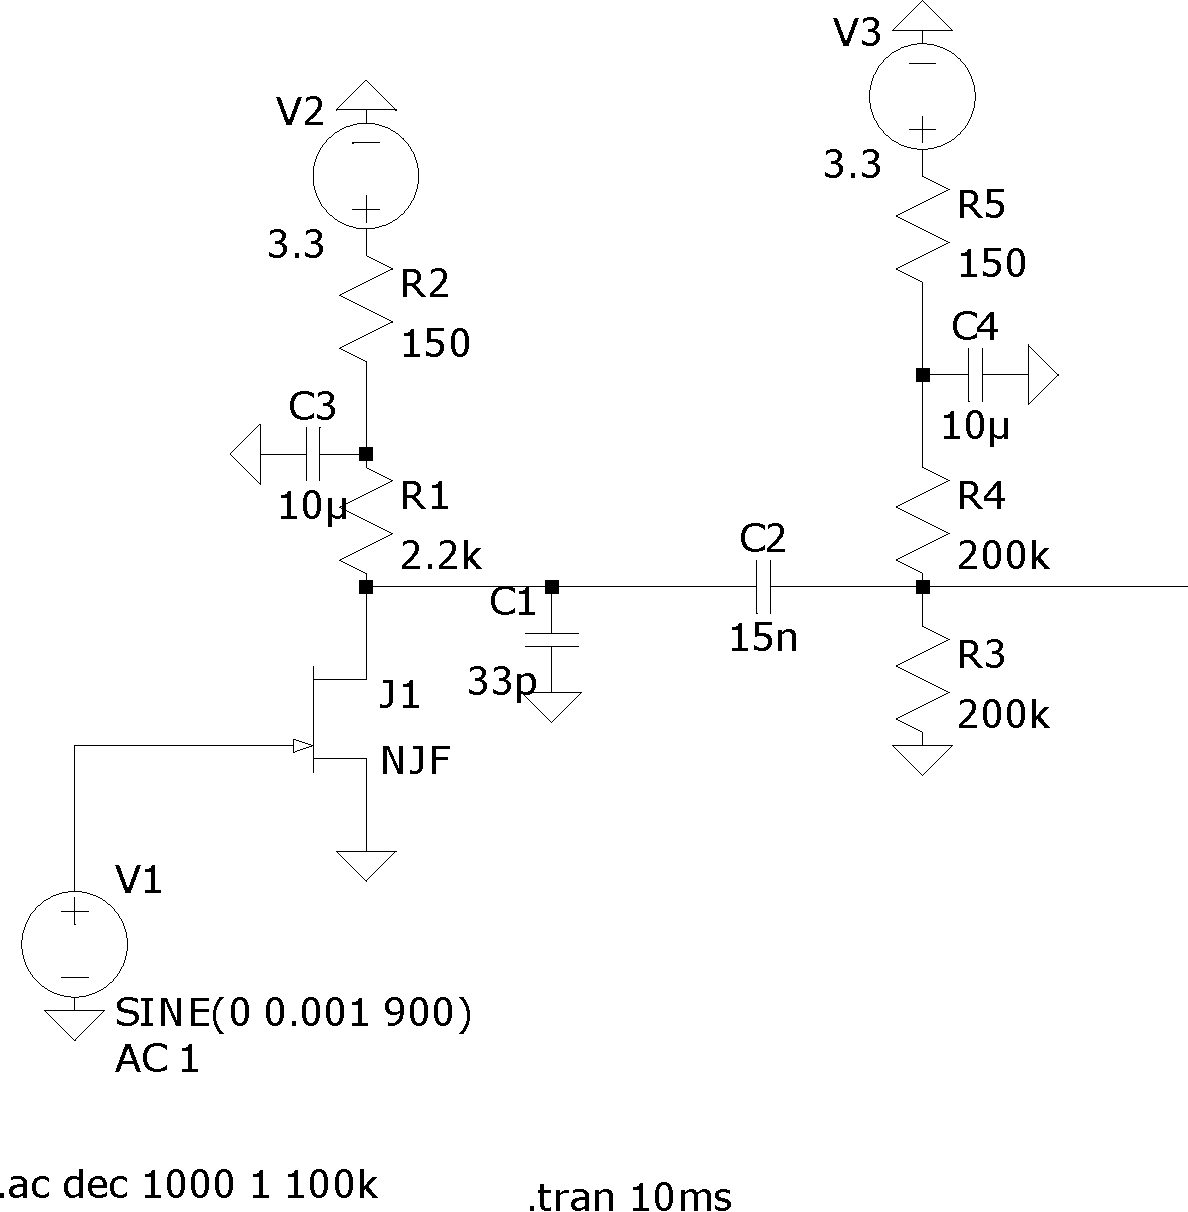
\includegraphics[width=0.4\textwidth]{pdffiles/HighPass/CircuitHighPassSimulationJET.pdf}
    \caption{Schéma de simulation sur LTspice du cas \textit{équivalent transistor}}
    \label{fig:ltspice_transistor}
\end{figure}



Après simulation, on obtient sur la figure \ref{fig:bodesim} les courbes de Bode des différents circuits. On remarque que les courbes ont toutes la même allure, avec une fréquence de coupure située aux alentours de $100 \ Hz$. Par ailleurs, dans la simulation avec transistor, le gain est en dessous de $ 0 \ dB$. Ce n'est pas un problème car ce qui nous intéresse est l'impact de la résistance de polarisation et des filtres passe-bas sur les caractéristiques du filtre passe-haut : \textbf{la fréquence de coupure}.

On en conclut que la résistance de polarisation et les filtres passe-bas ont une influence négligeable sur les caractéristiques du filtre passe-haut.



\begin{figure}[H]
    \centering
    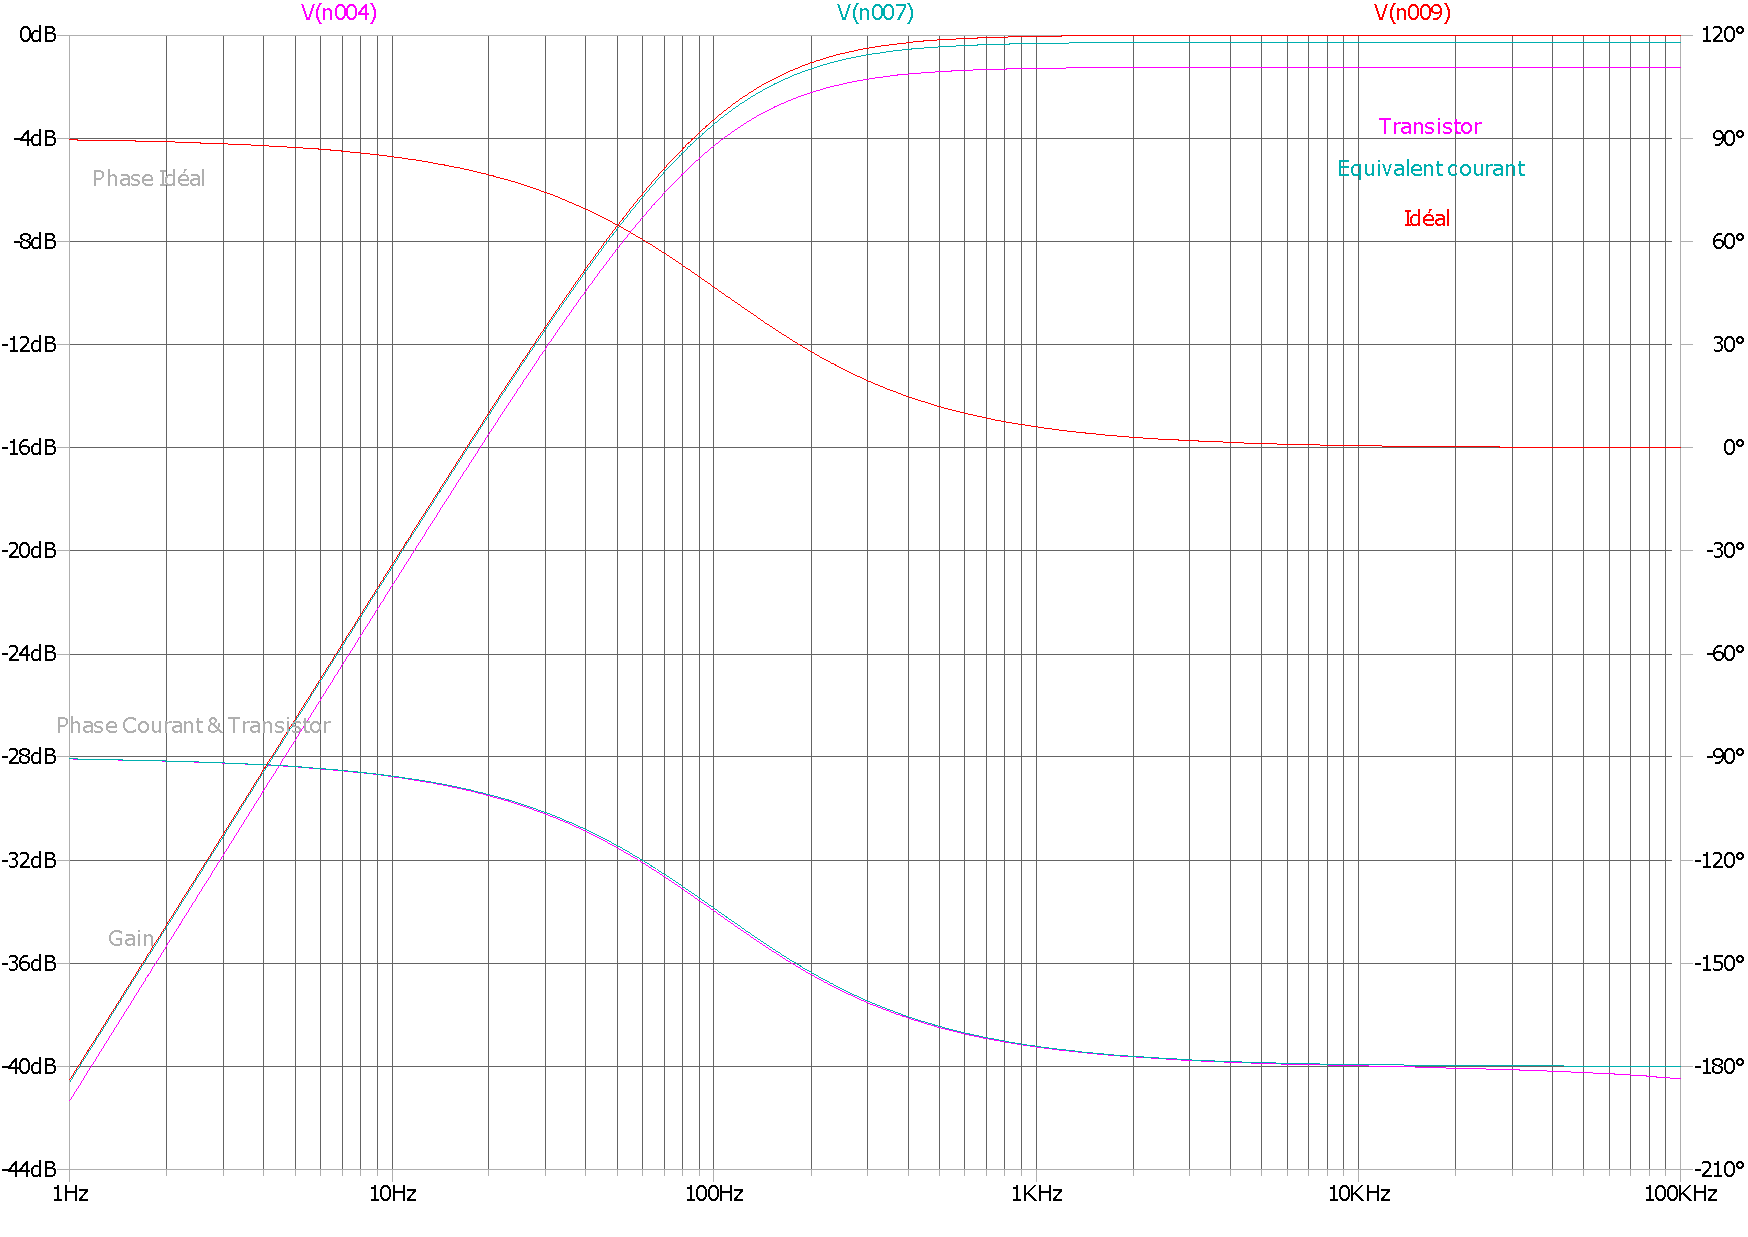
\includegraphics[width=\textwidth]{pdffiles/HighPass/BodeHighPassImpactePolarisation.pdf}
    \caption{Courbe de Bode du filtre passe-haut dans différent cas. Cas \textit{idéal} en rouge, cas \textit{équivalent courant} en bleu et cas \textit{équivalent transistor} en rose }
    \label{fig:bodesim}
\end{figure}

\subsubsection{Critique sur le gain maximal en simulation}

Sachant qu'on ne peut pas obtenir la courbe de Bode de la chaîne d'acquisition à partir du Picoscope, on a décidé de l'obtenir à l'aide de LTspice, en faisant deux simulations. Dans la première, le microphone est remplacé par son équivalent transistor et dans la deuxième par son équivalent source de courant. Pour plus de détails à propos de la simulation et pour voir toutes les courbes, allez voir l'Annexe \ref{Bodechaineacquiannexe}

La figure \ref{fig:BodeFullCircuitJet} est la courbe obtenue dans le premier cas, qui est le pire, et on se rend compte qu'on n'atteint pas le gain voulu. En effet, on peut voir que le gain à $1100 \ Hz$ est de $61.58 \ dB$. Pour rappel, le gain souhaité est de $64.35 \ dB$. 
De manière plus générale, il y aura toujours une différence entre le gain souhaité et le gain réel.

\begin{figure}[H]
    \centering
    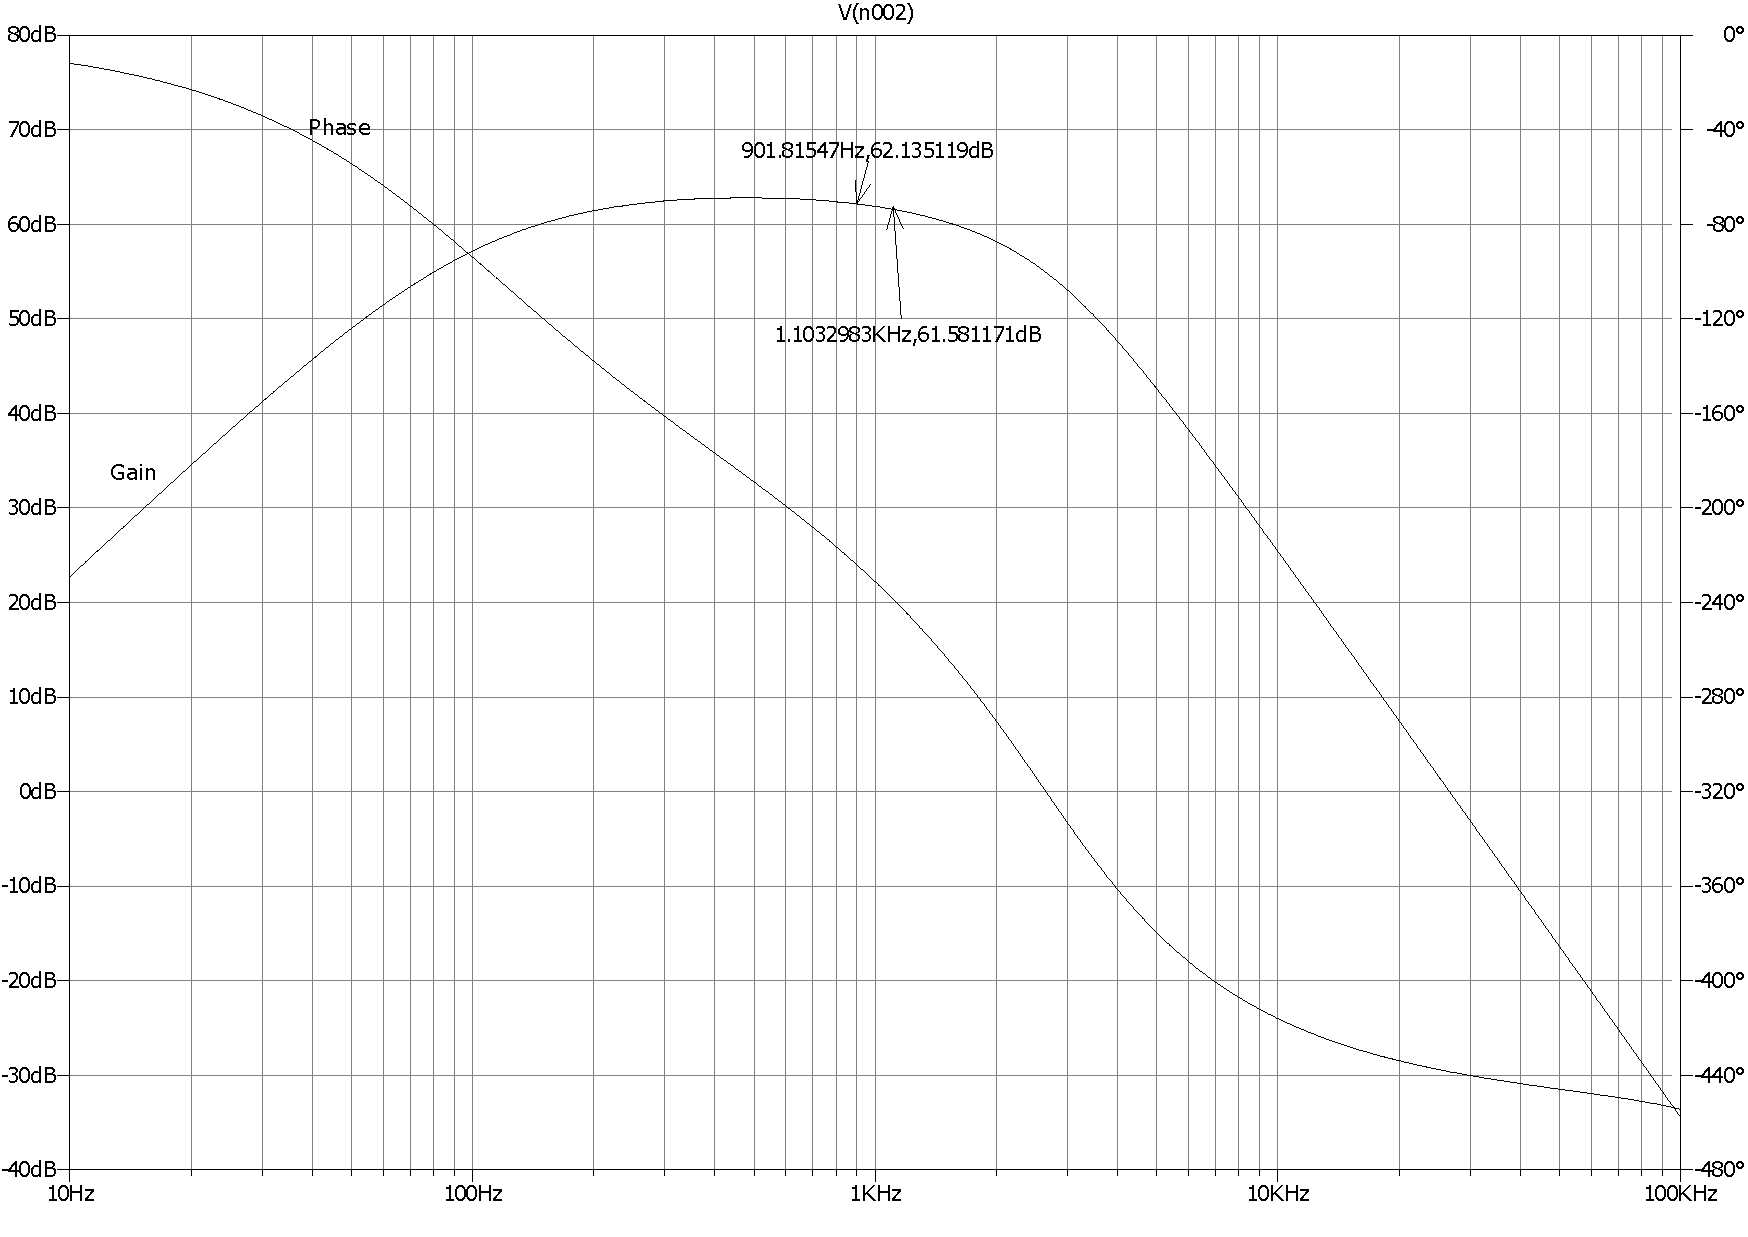
\includegraphics[width=\textwidth]{pdffiles/BodeCircuitJET.pdf}
    \caption{Courbe de Bode de la chaîne d'acquisition. Le microphone est remplacé par son équivalent transistor}
    \label{fig:BodeFullCircuitJet}
\end{figure}

Nous avons décidé de ne rien changer mais on peut toujours rajouter une petite marge en augmentant le gain de l'étage d'amplification. C'est faisable car le gain maximal à $1100 \ Hz$ en un seul étage est de $68.11 \ dB$. Attention cependant à ne pas trop l'augmenter, on veut éviter la saturation.